\documentclass[12pt,a4paper]{article}
\usepackage[UTF-8]{inputenc}
\usepackage{natbib,geometry,subfigure,float}
\usepackage{ifthen,amsmath,amssymb,amsthm,bm,graphicx,color,ctex,fancyhdr}
\geometry{a4paper,top=2cm,bottom=3cm,left=3cm,right=3cm}
\pagestyle{fancy}
\renewcommand{\headrulewidth}{0pt}
\renewcommand{\baselinestretch}{1} % 行距为当前正文字体的1.5倍
\title{Anti-aliasing}
\date{}
\author{}
\begin{document}
\maketitle
1. The figure that we have is an RGB figure. To sample it, we use $rgb2gray()$ function to gray it, then sampled with
frequency 2,4,8.
\begin{figure}[H]
    \centering  %图片全局居中
    \subfigure[original]{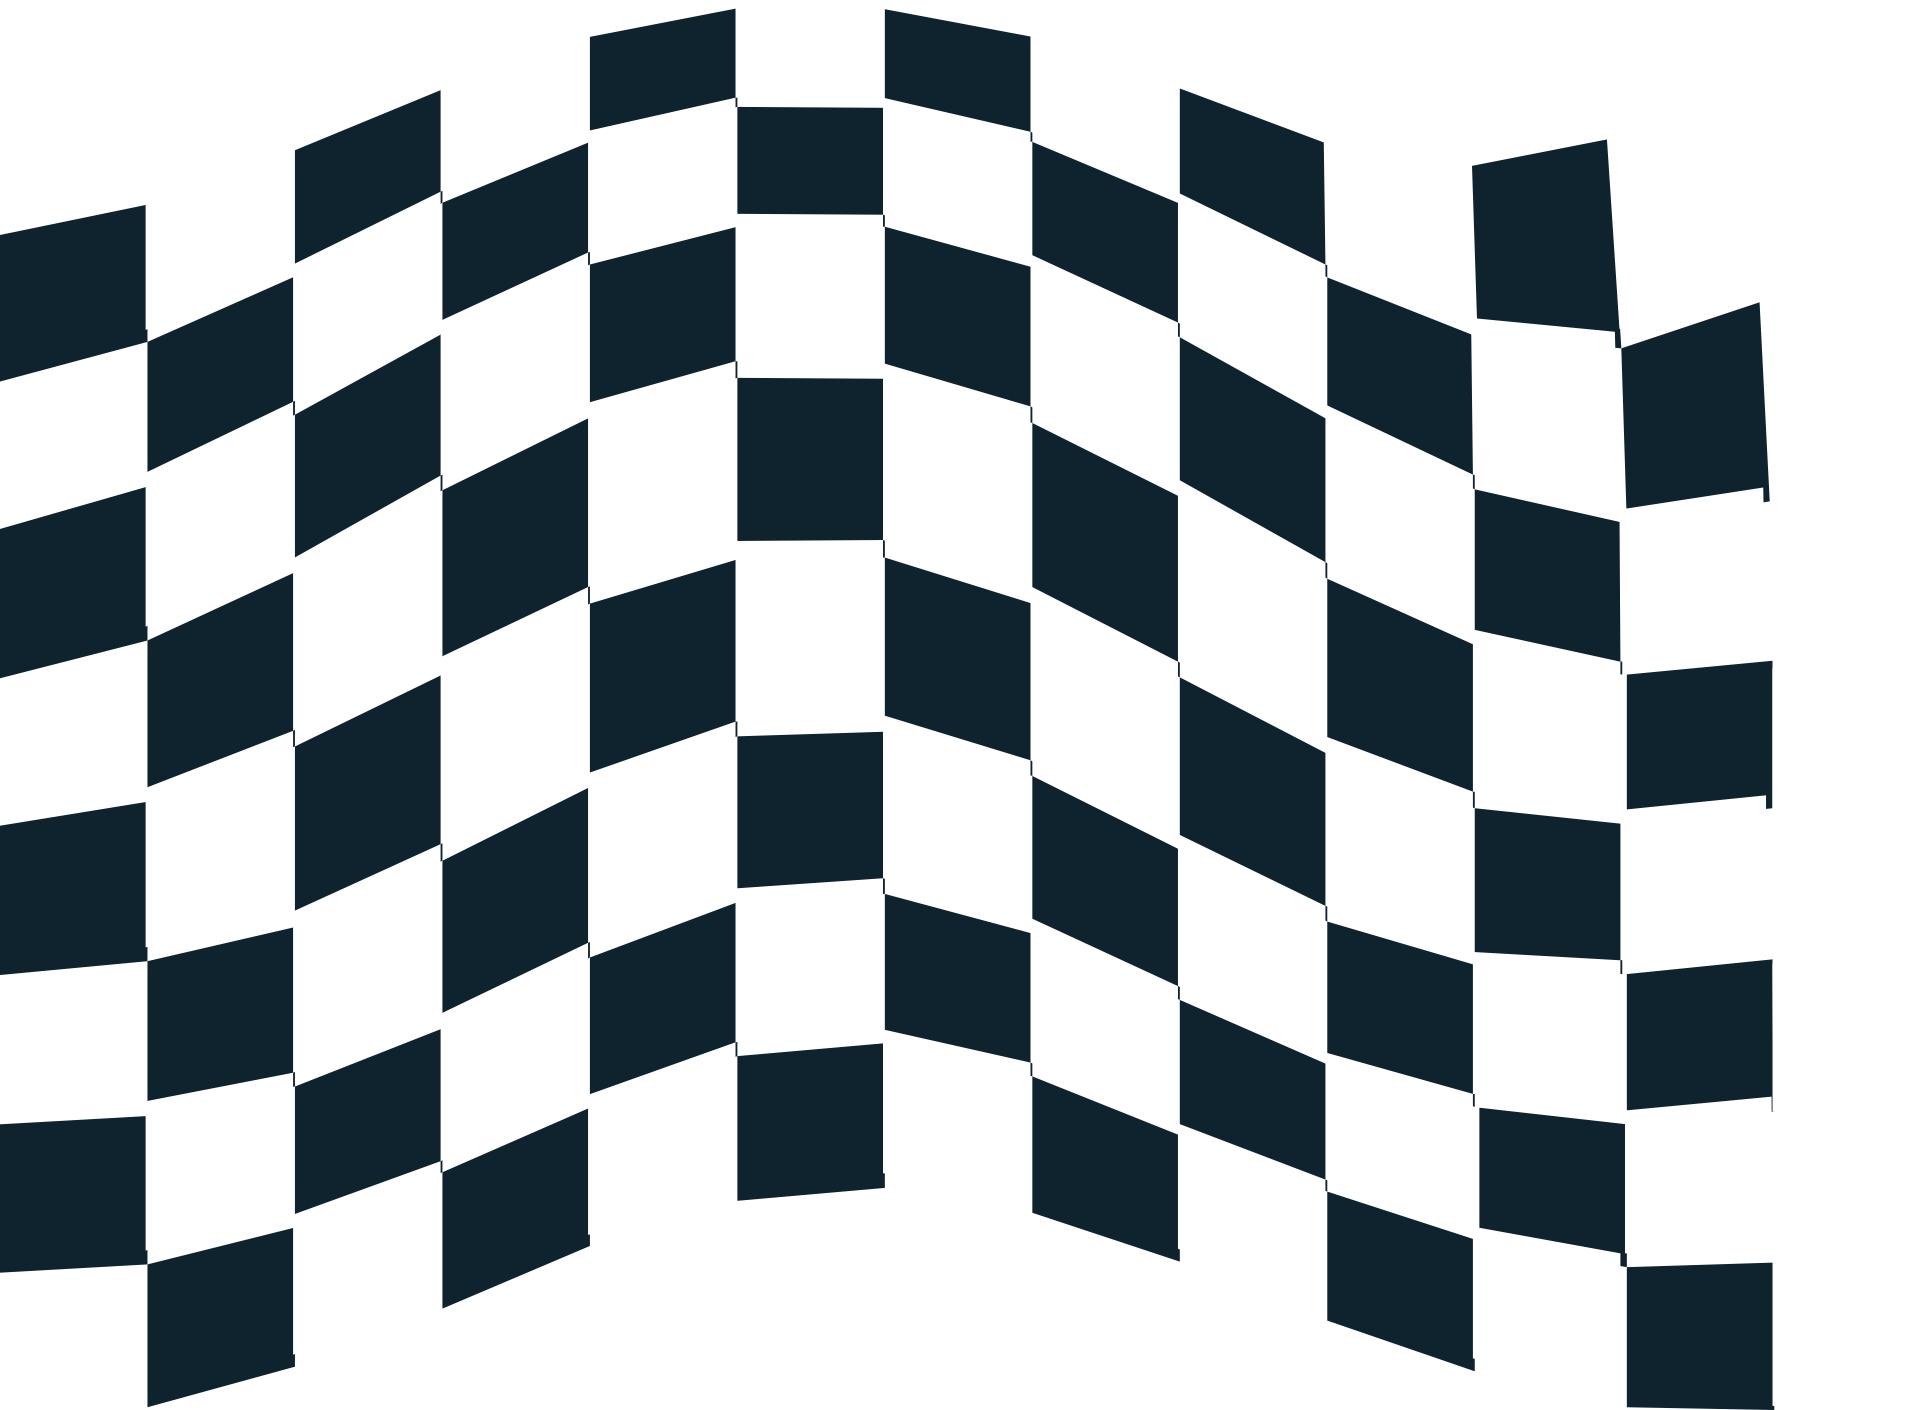
\includegraphics[scale=0.09]{original.png}}
    \subfigure[gray]{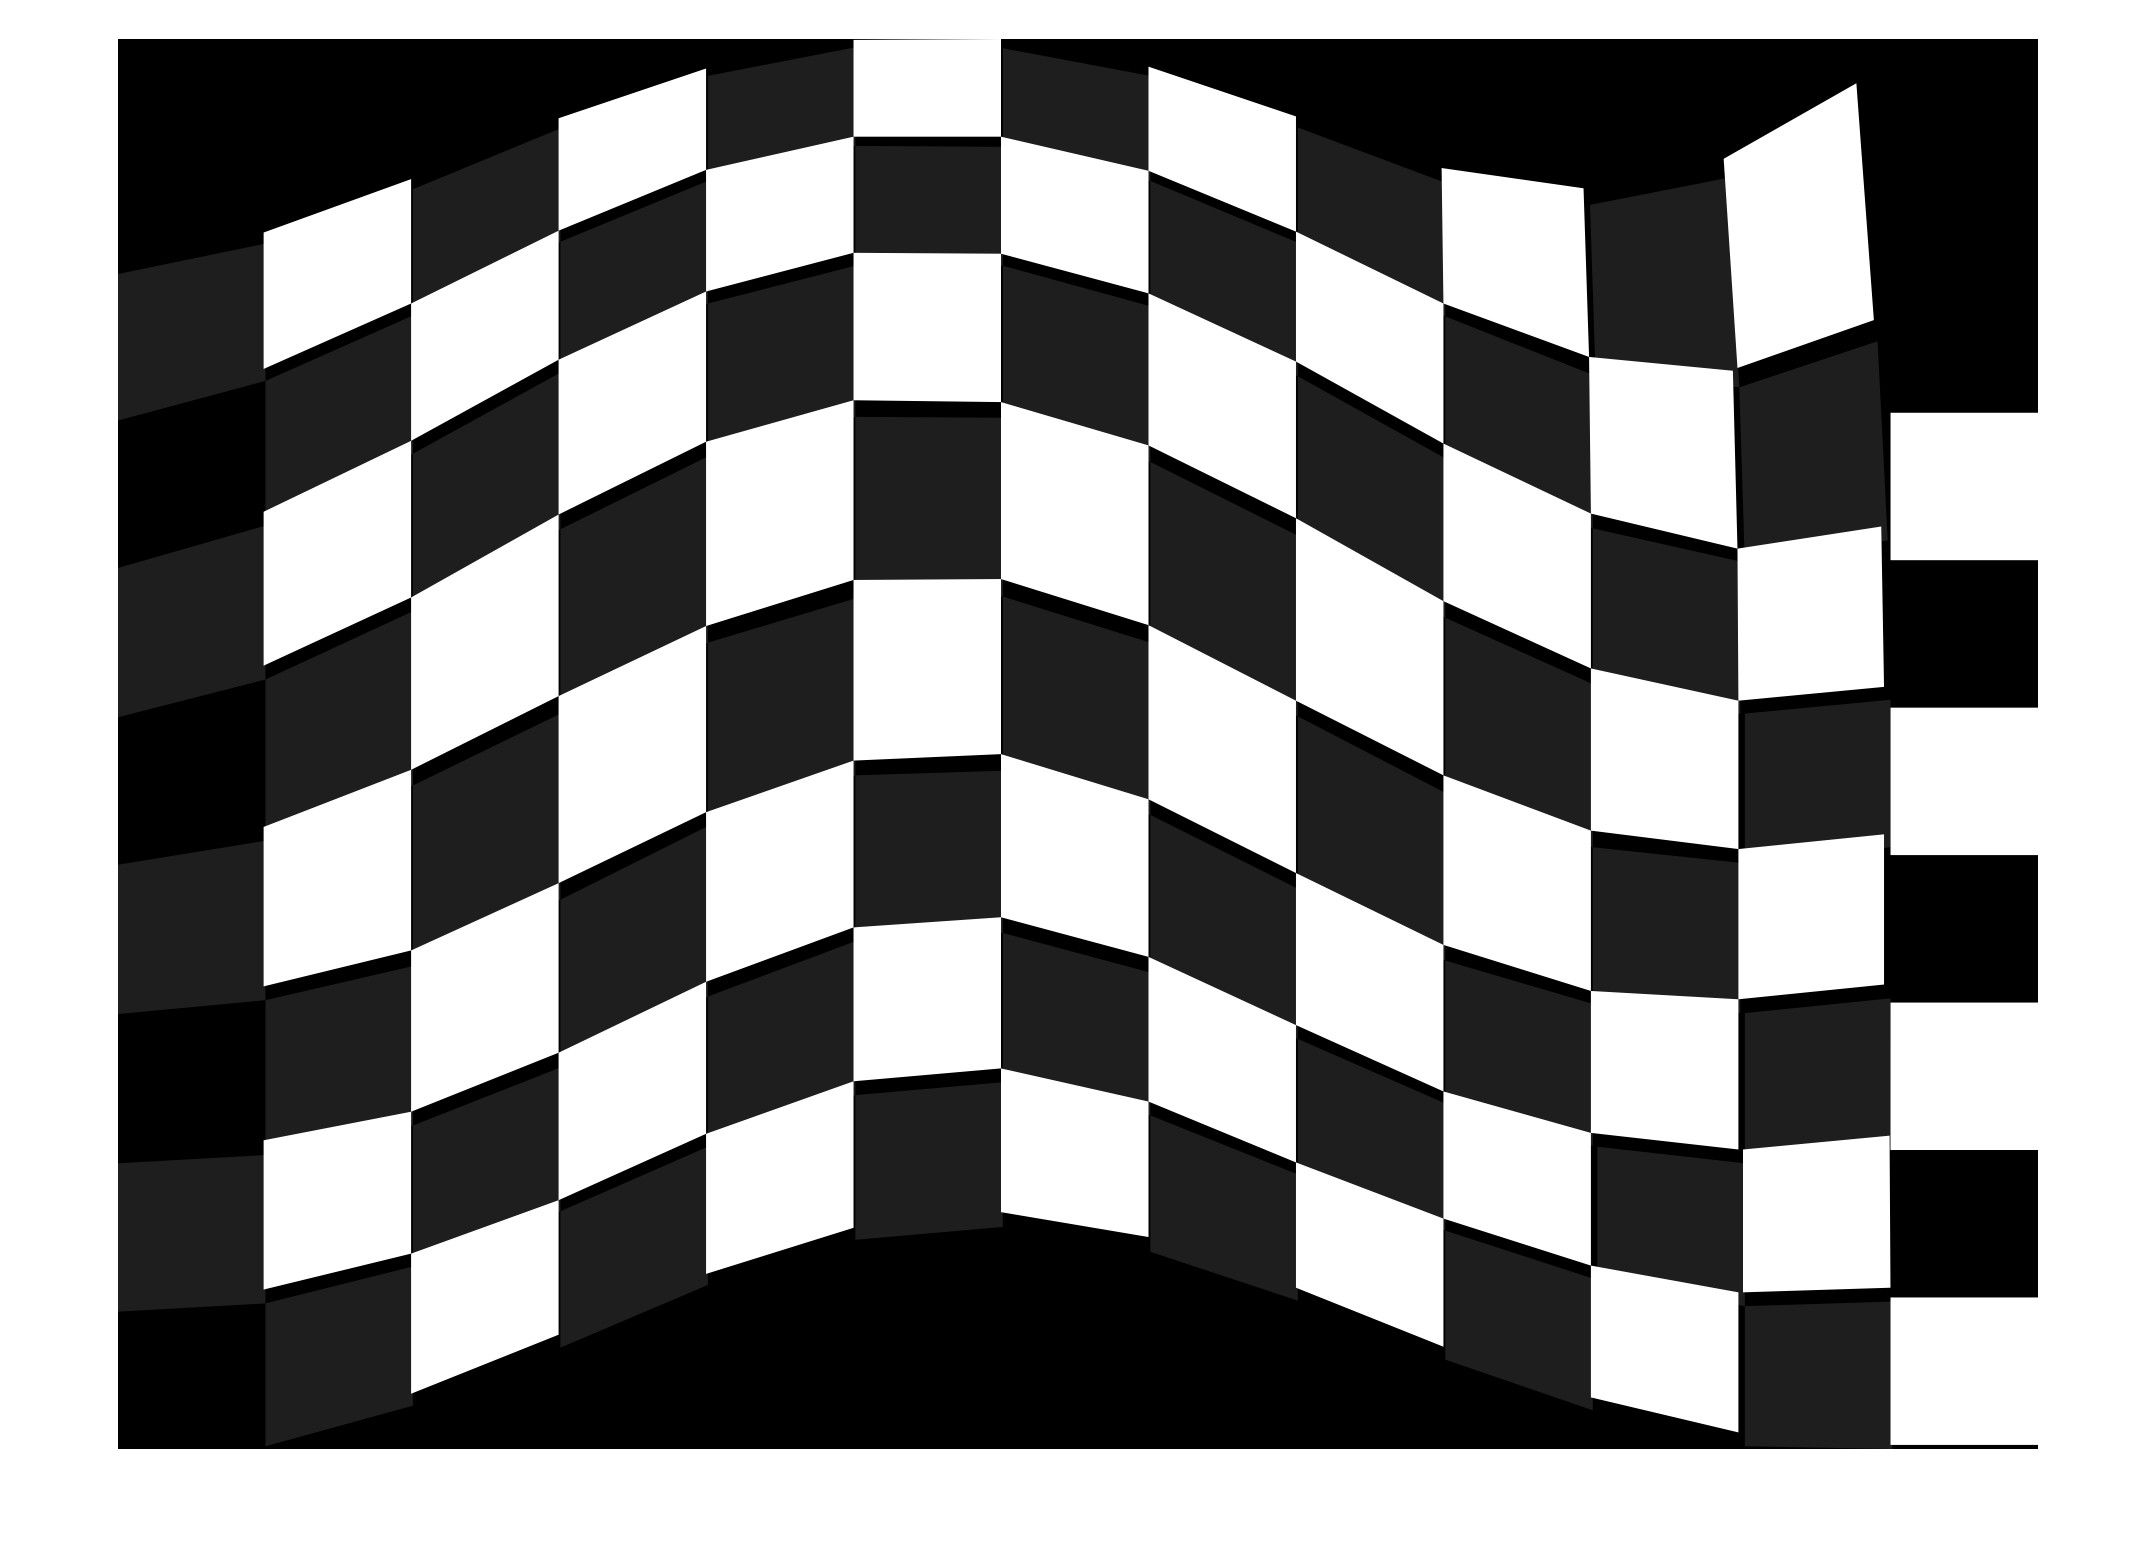
\includegraphics[scale=0.09]{Original_gray_pic.jpg}}
    \subfigure[f=4]{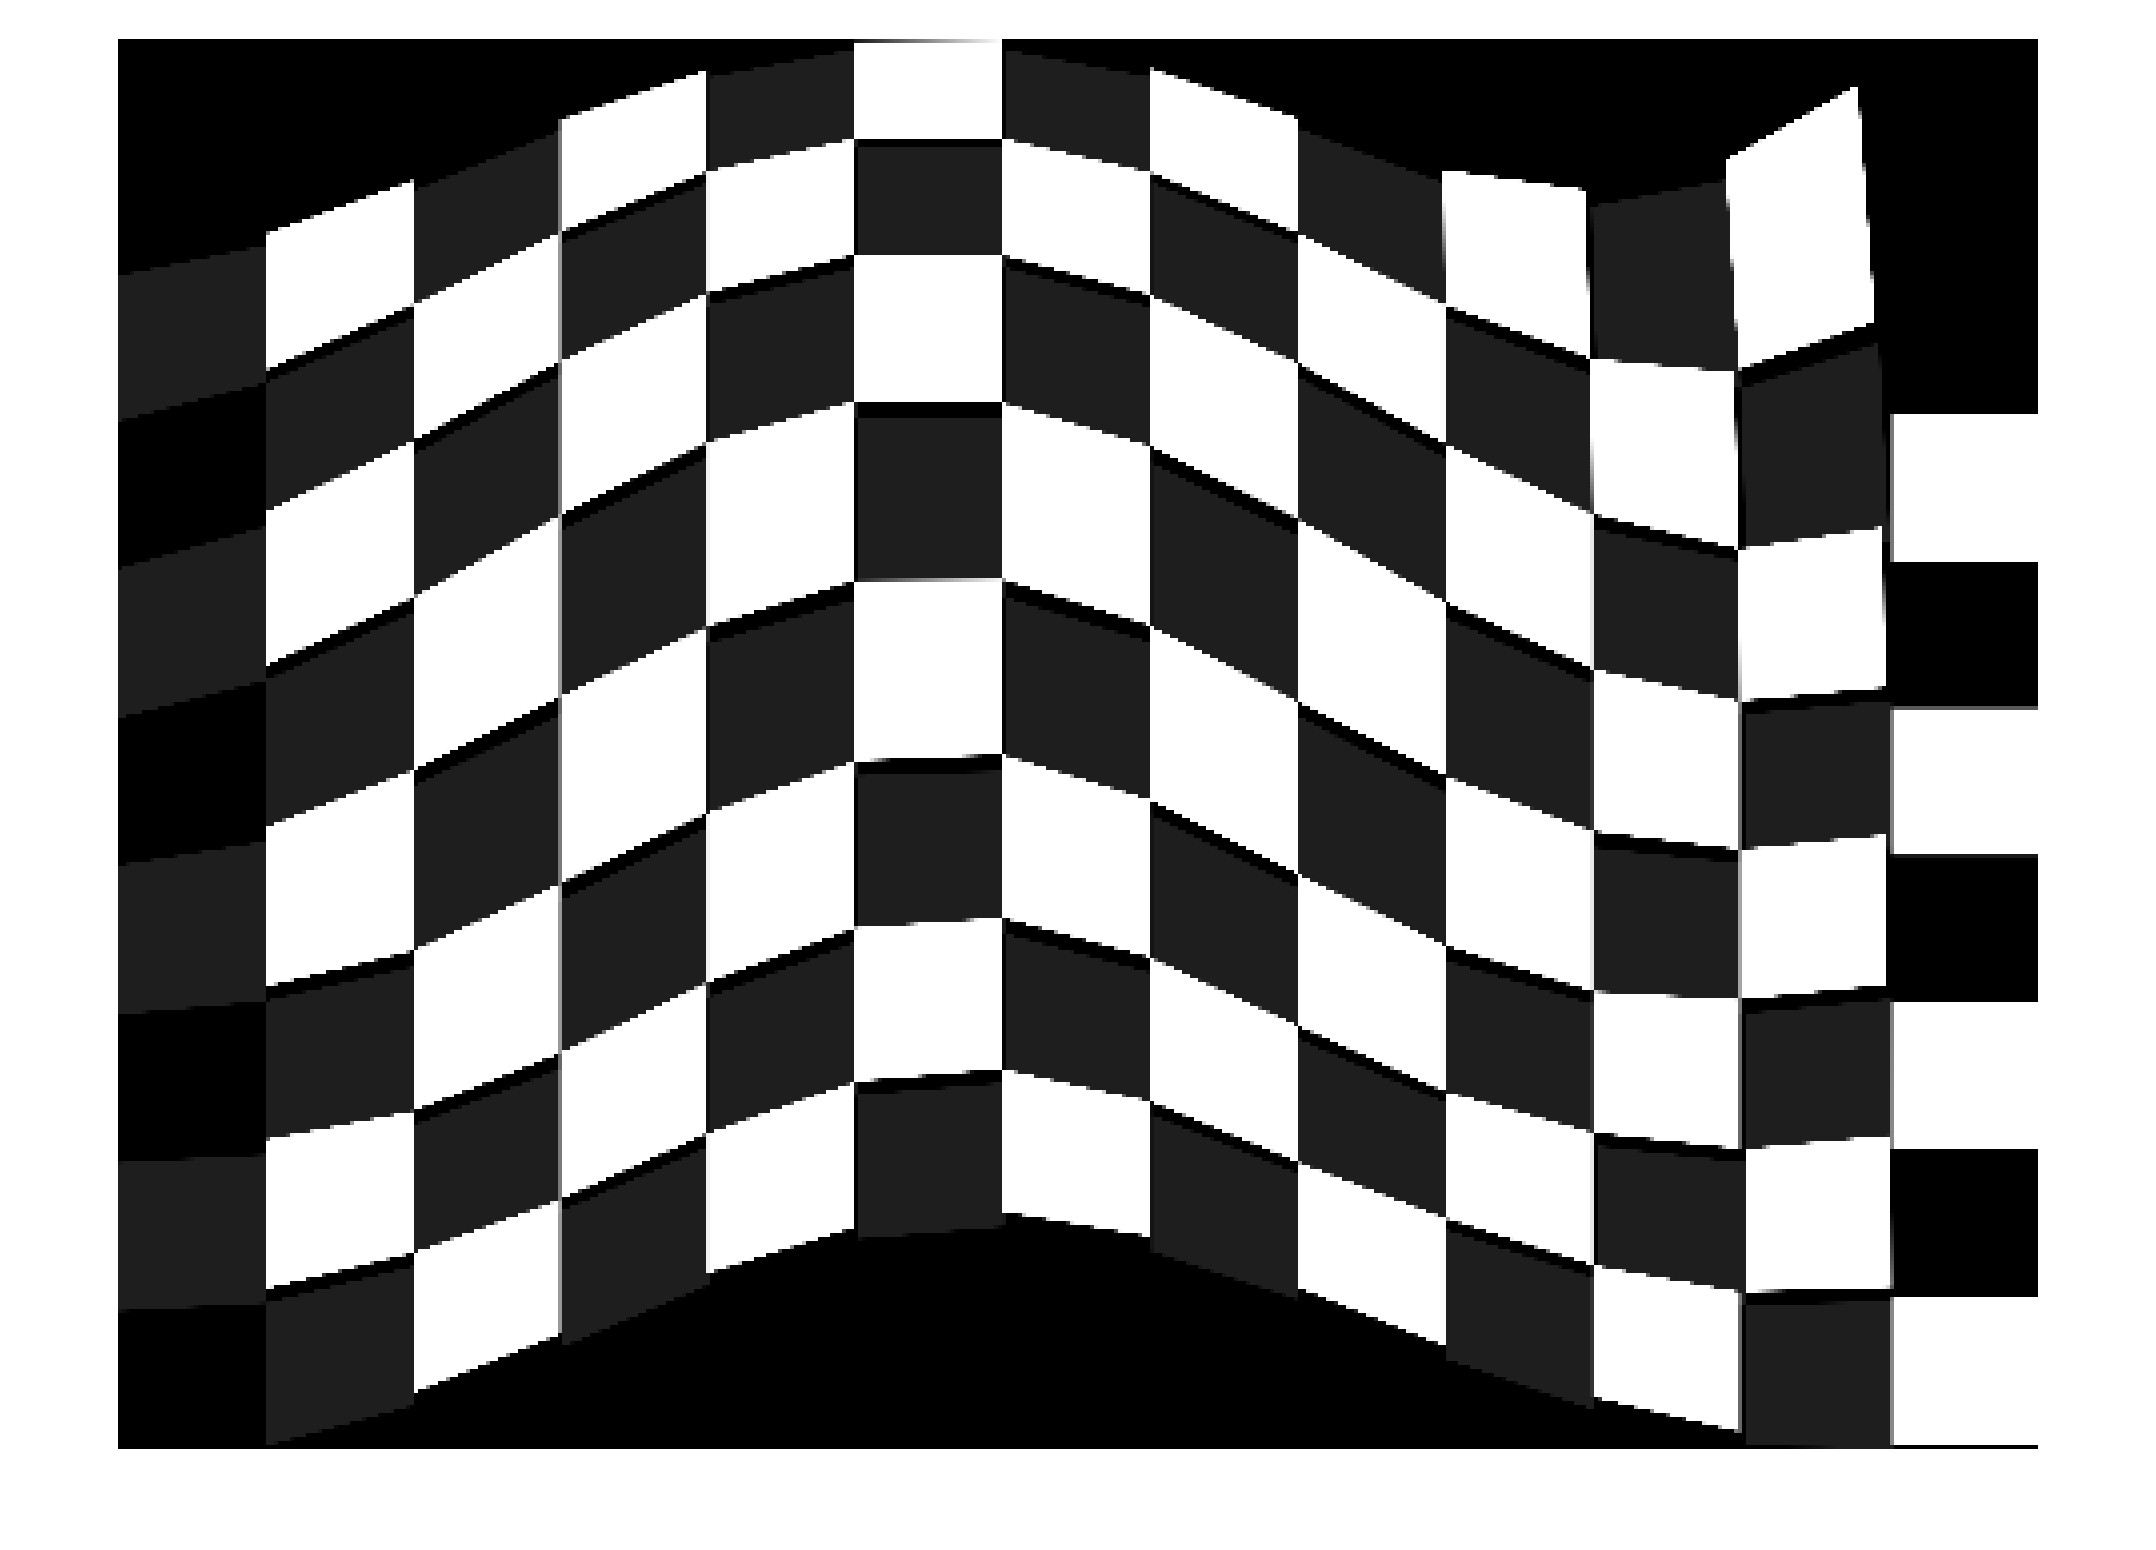
\includegraphics[scale=0.09]{Sampling_with_4.jpg}}
    \subfigure[f=8]{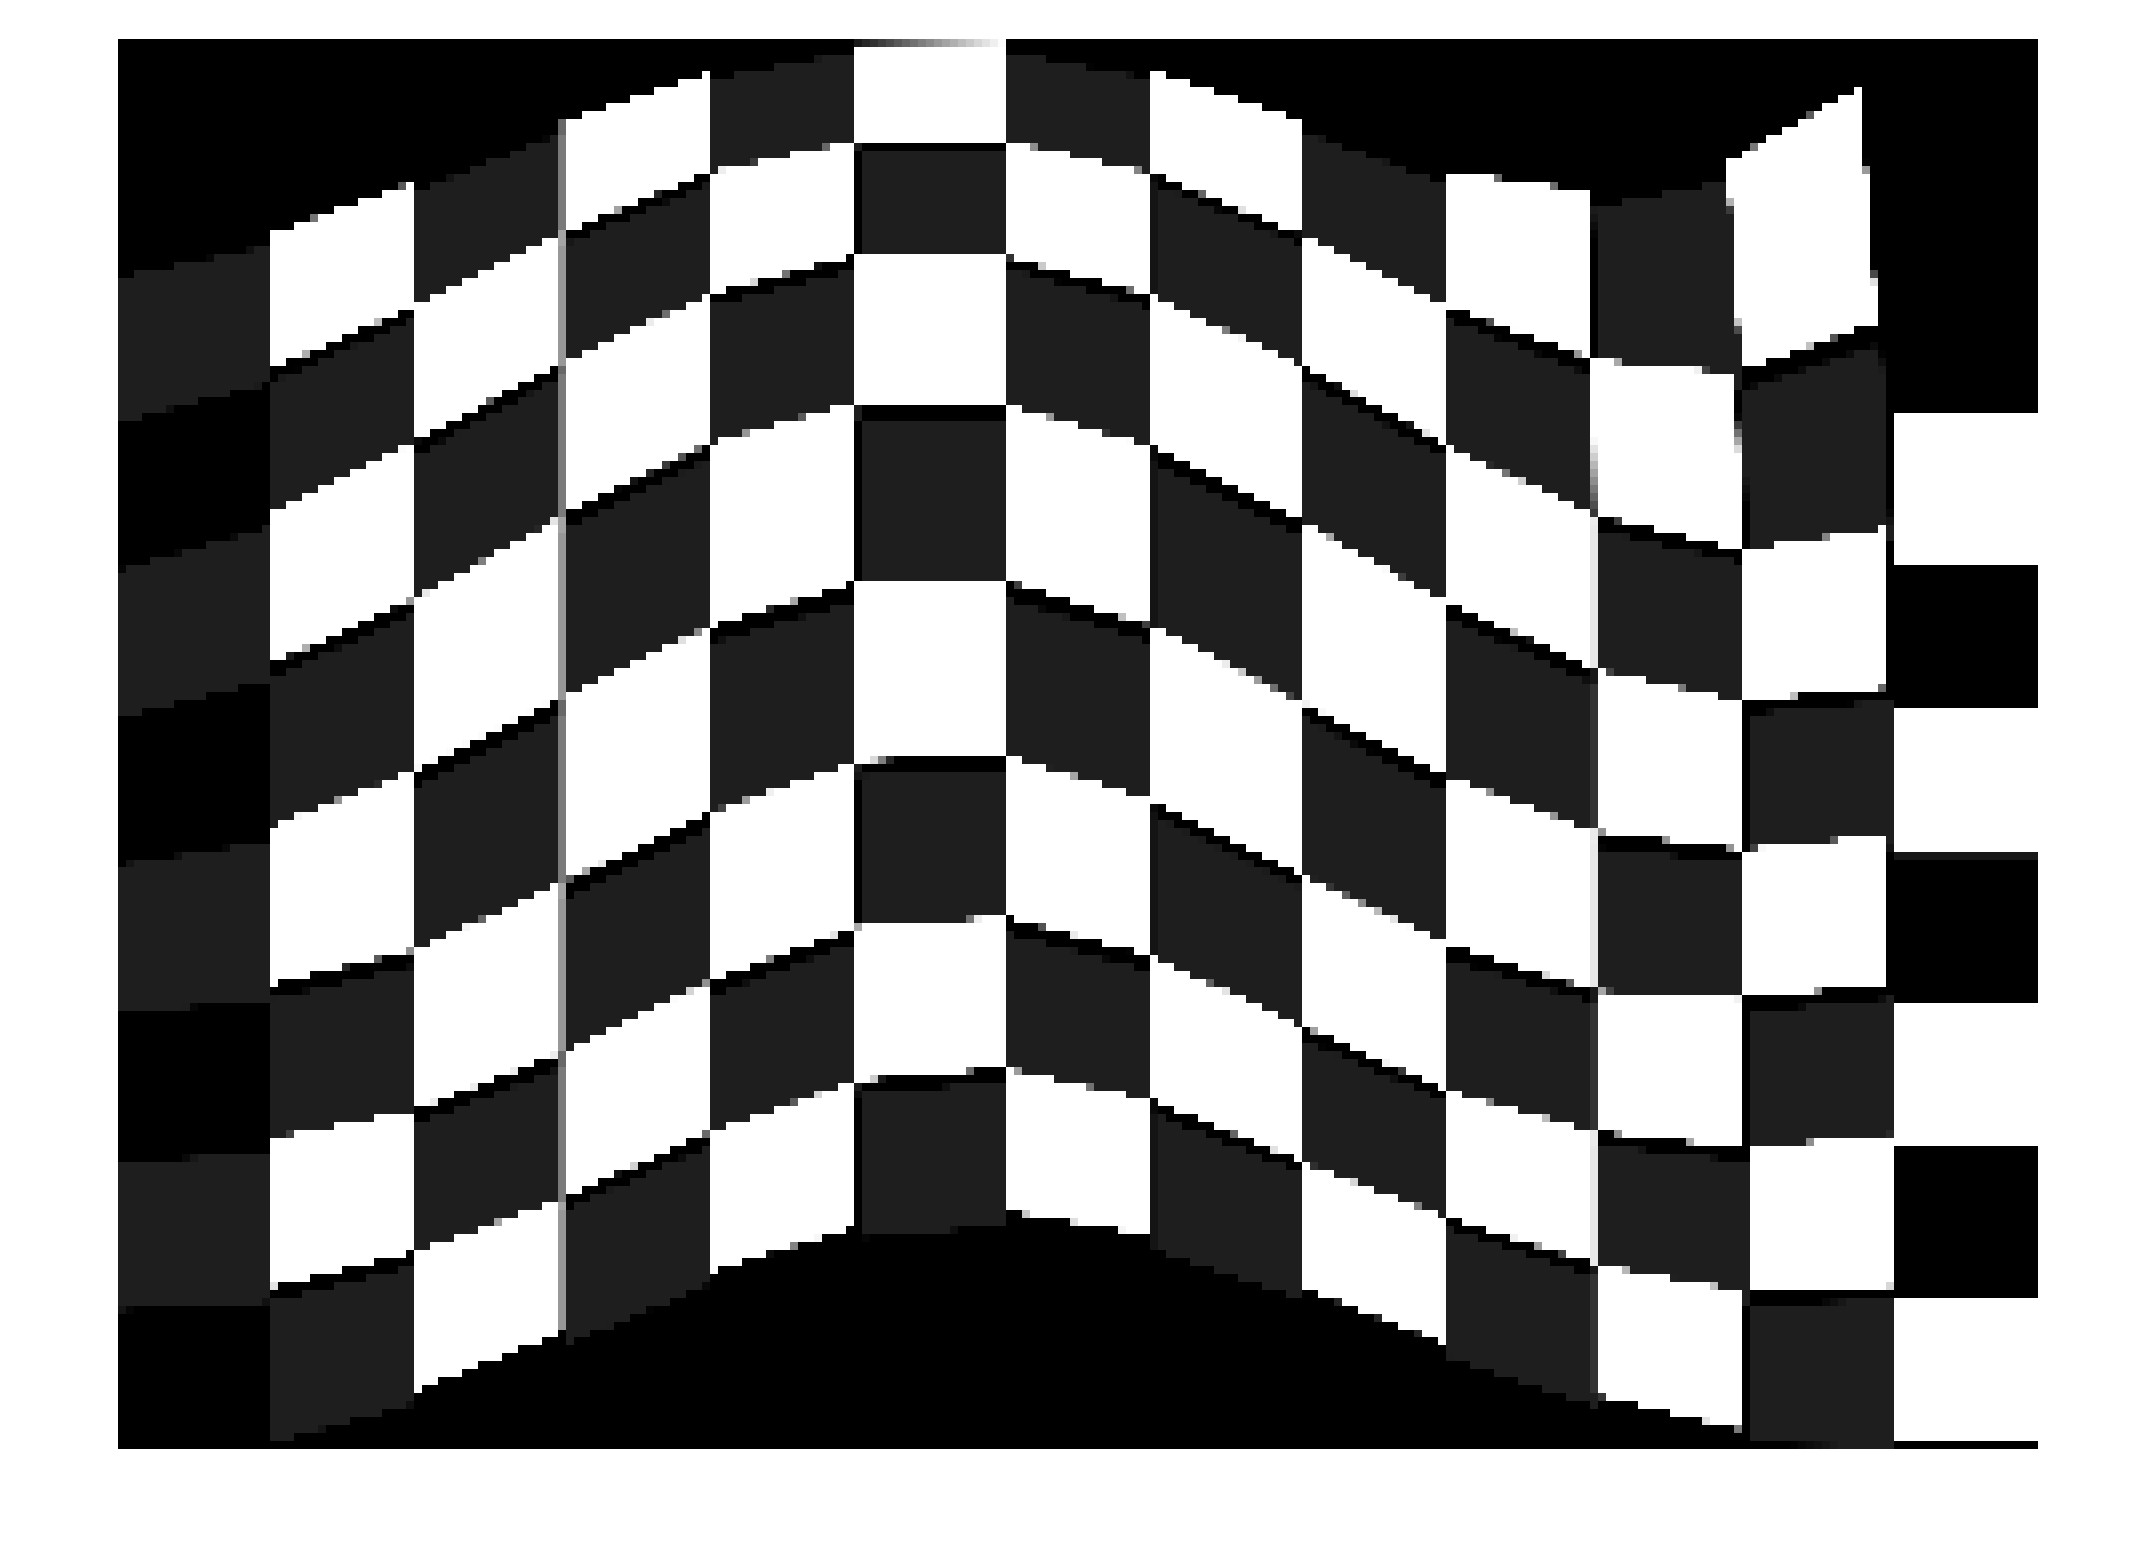
\includegraphics[scale=0.09]{Sampling_with_8.jpg}}
\end{figure}
For f=8,it is obviously that we can see aliasing, the edge of the graph is jaggy.
But before we filter, let us take a look at different interpolation method on f=8.\par
2. Interpolation: In the following experiments, we tested different interpolation method to see 
how the differences between each graph effects the resize.\par
In the following experiment, we use nearest, bilinear, bicubic and box to interpolate the graph
to resize them to original size.

\clearpage

\begin{figure}[H]
    \centering  %图片全局居中
    \subfigure[nearest]{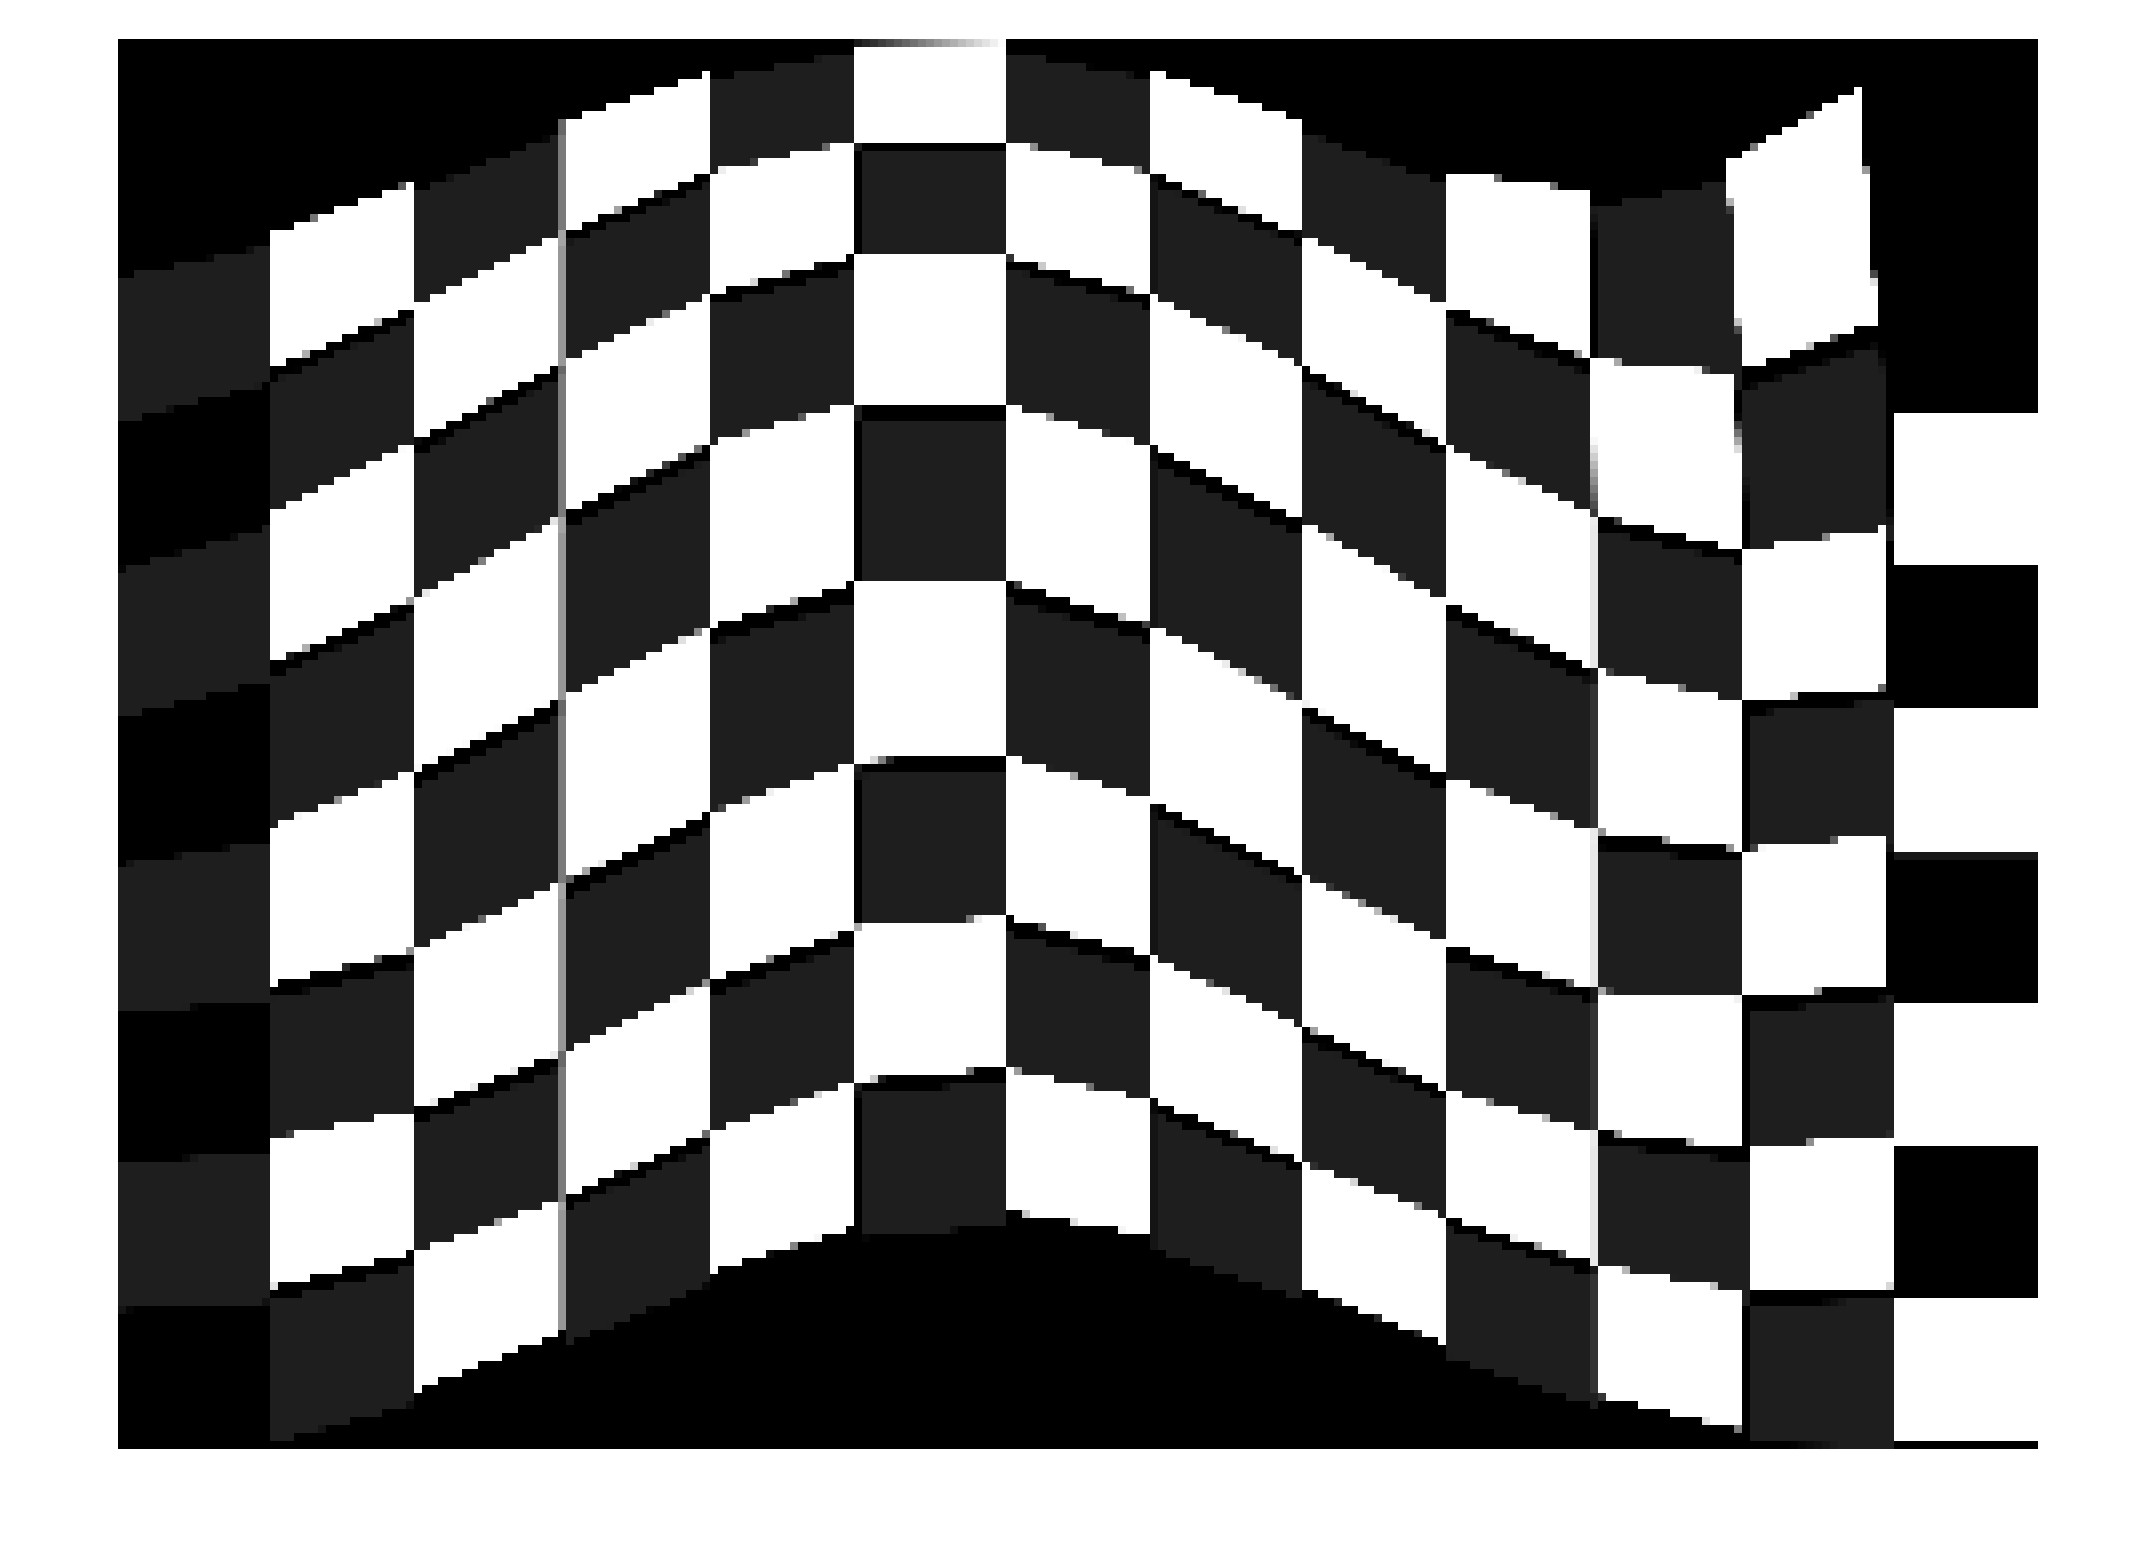
\includegraphics[scale=0.09]{interpolation_nearest.jpg}}
    \subfigure[bilinear]{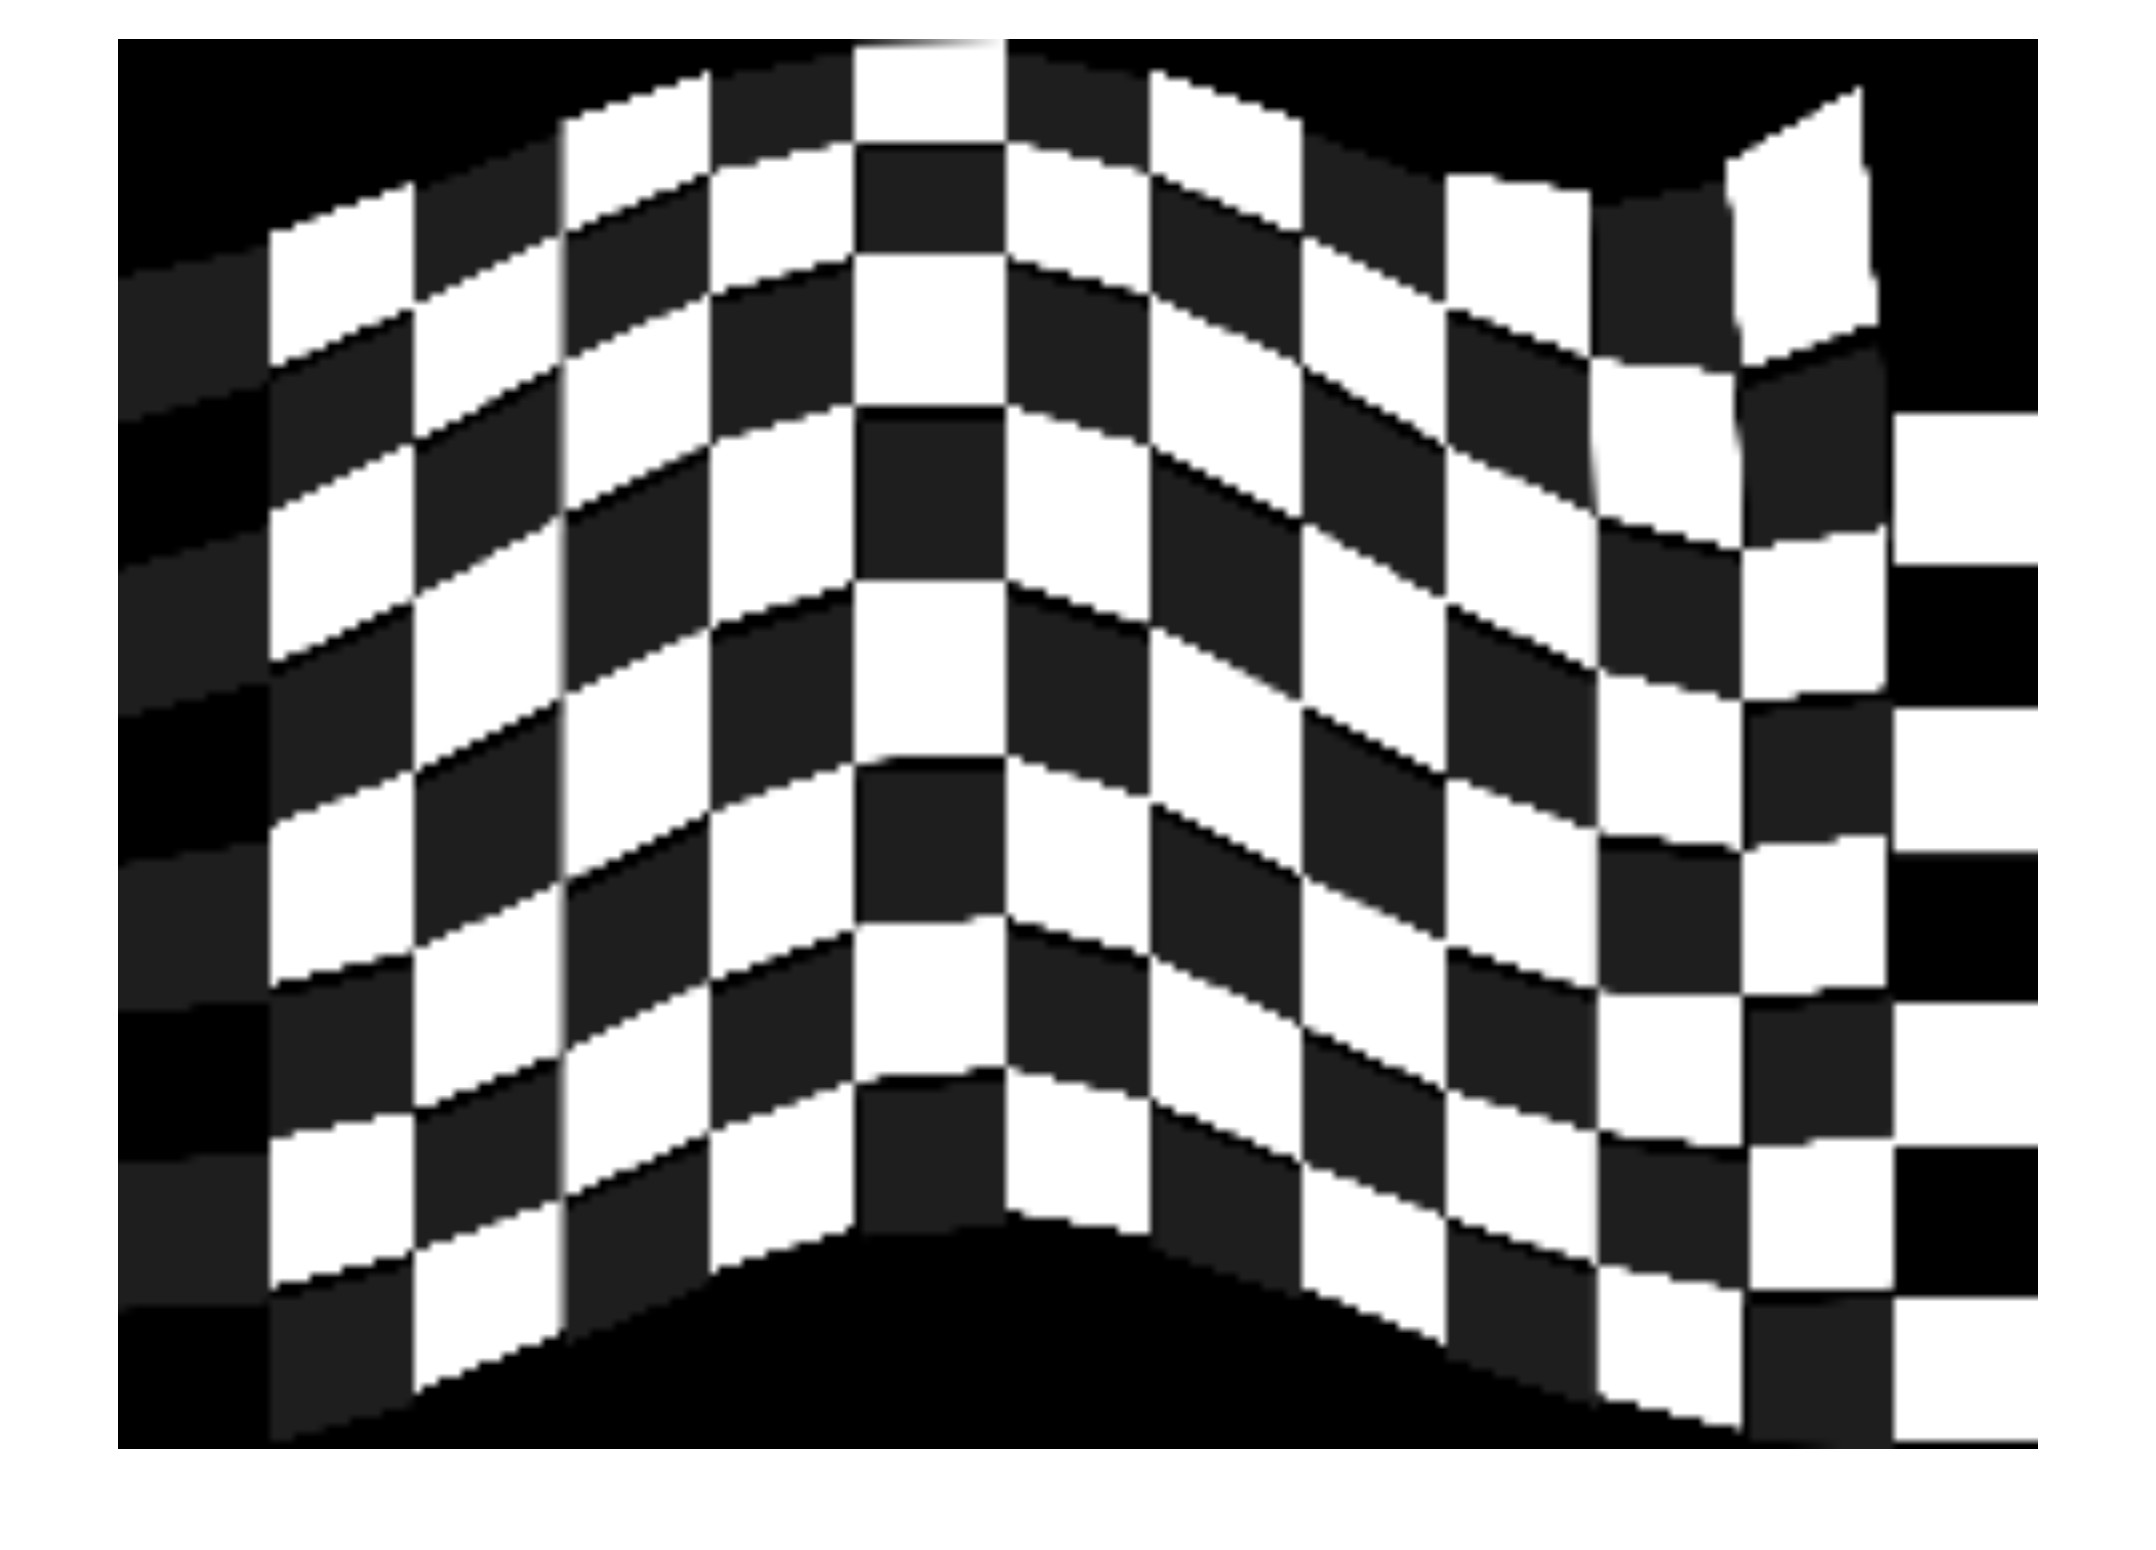
\includegraphics[scale=0.09]{interpolation_bilinear.jpg}}
    \subfigure[bicubic]{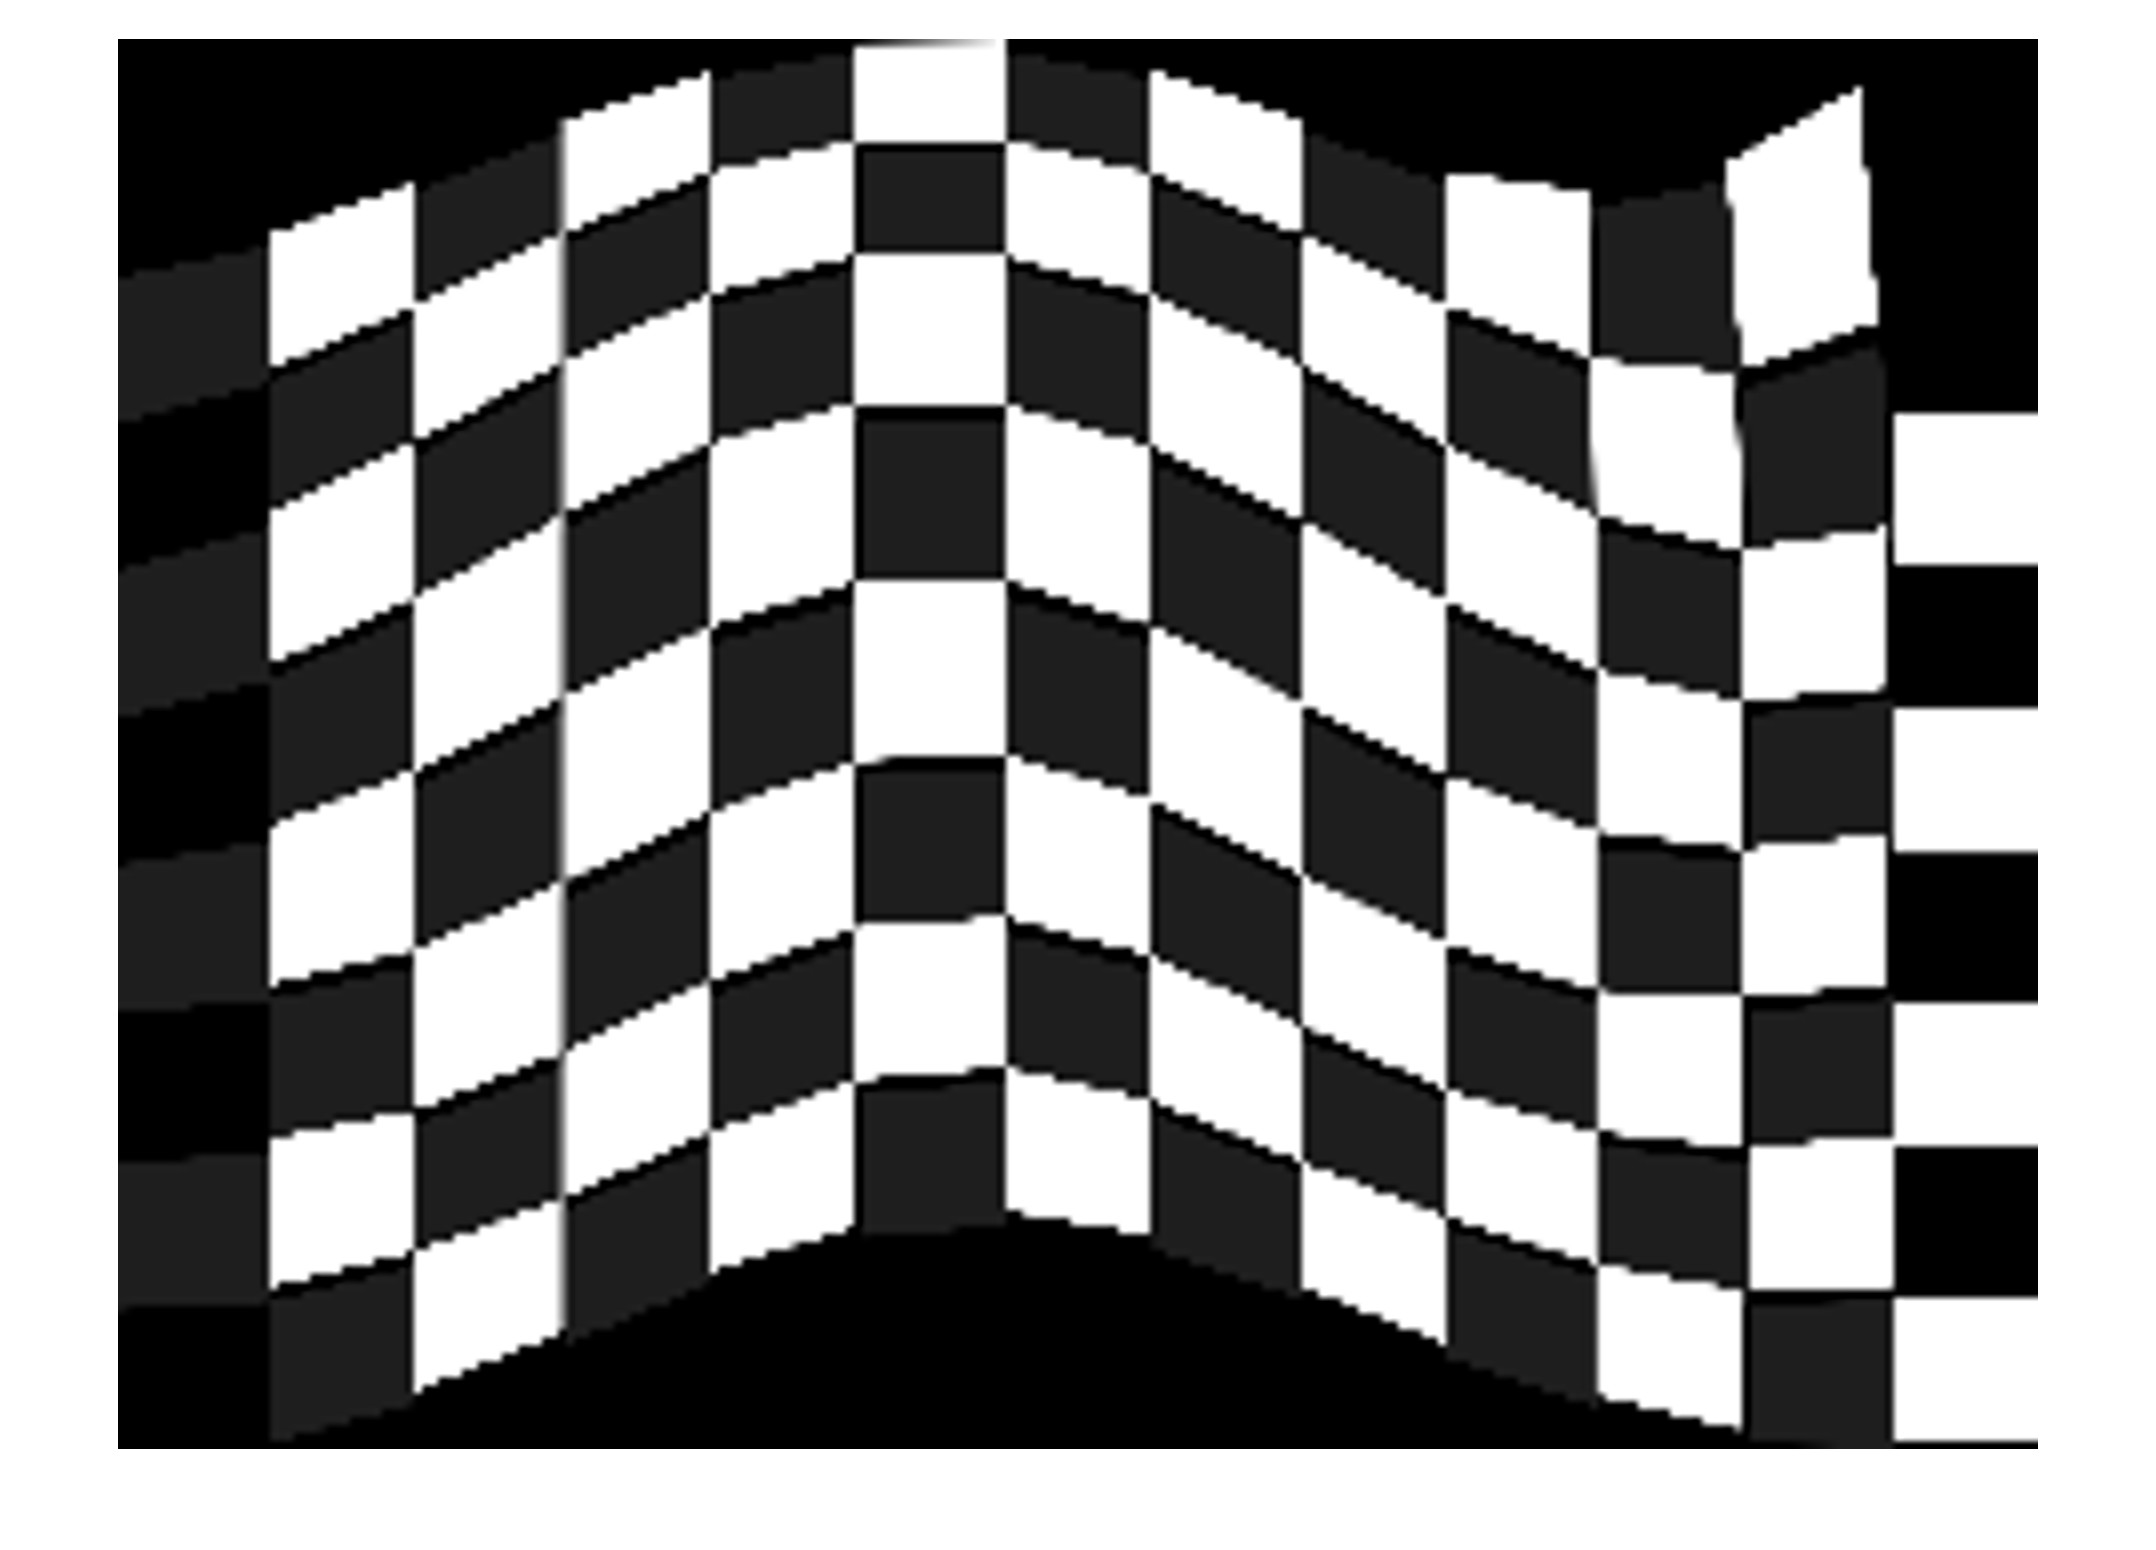
\includegraphics[scale=0.09]{interpolation_bicubic.jpg}}
    \subfigure[box]{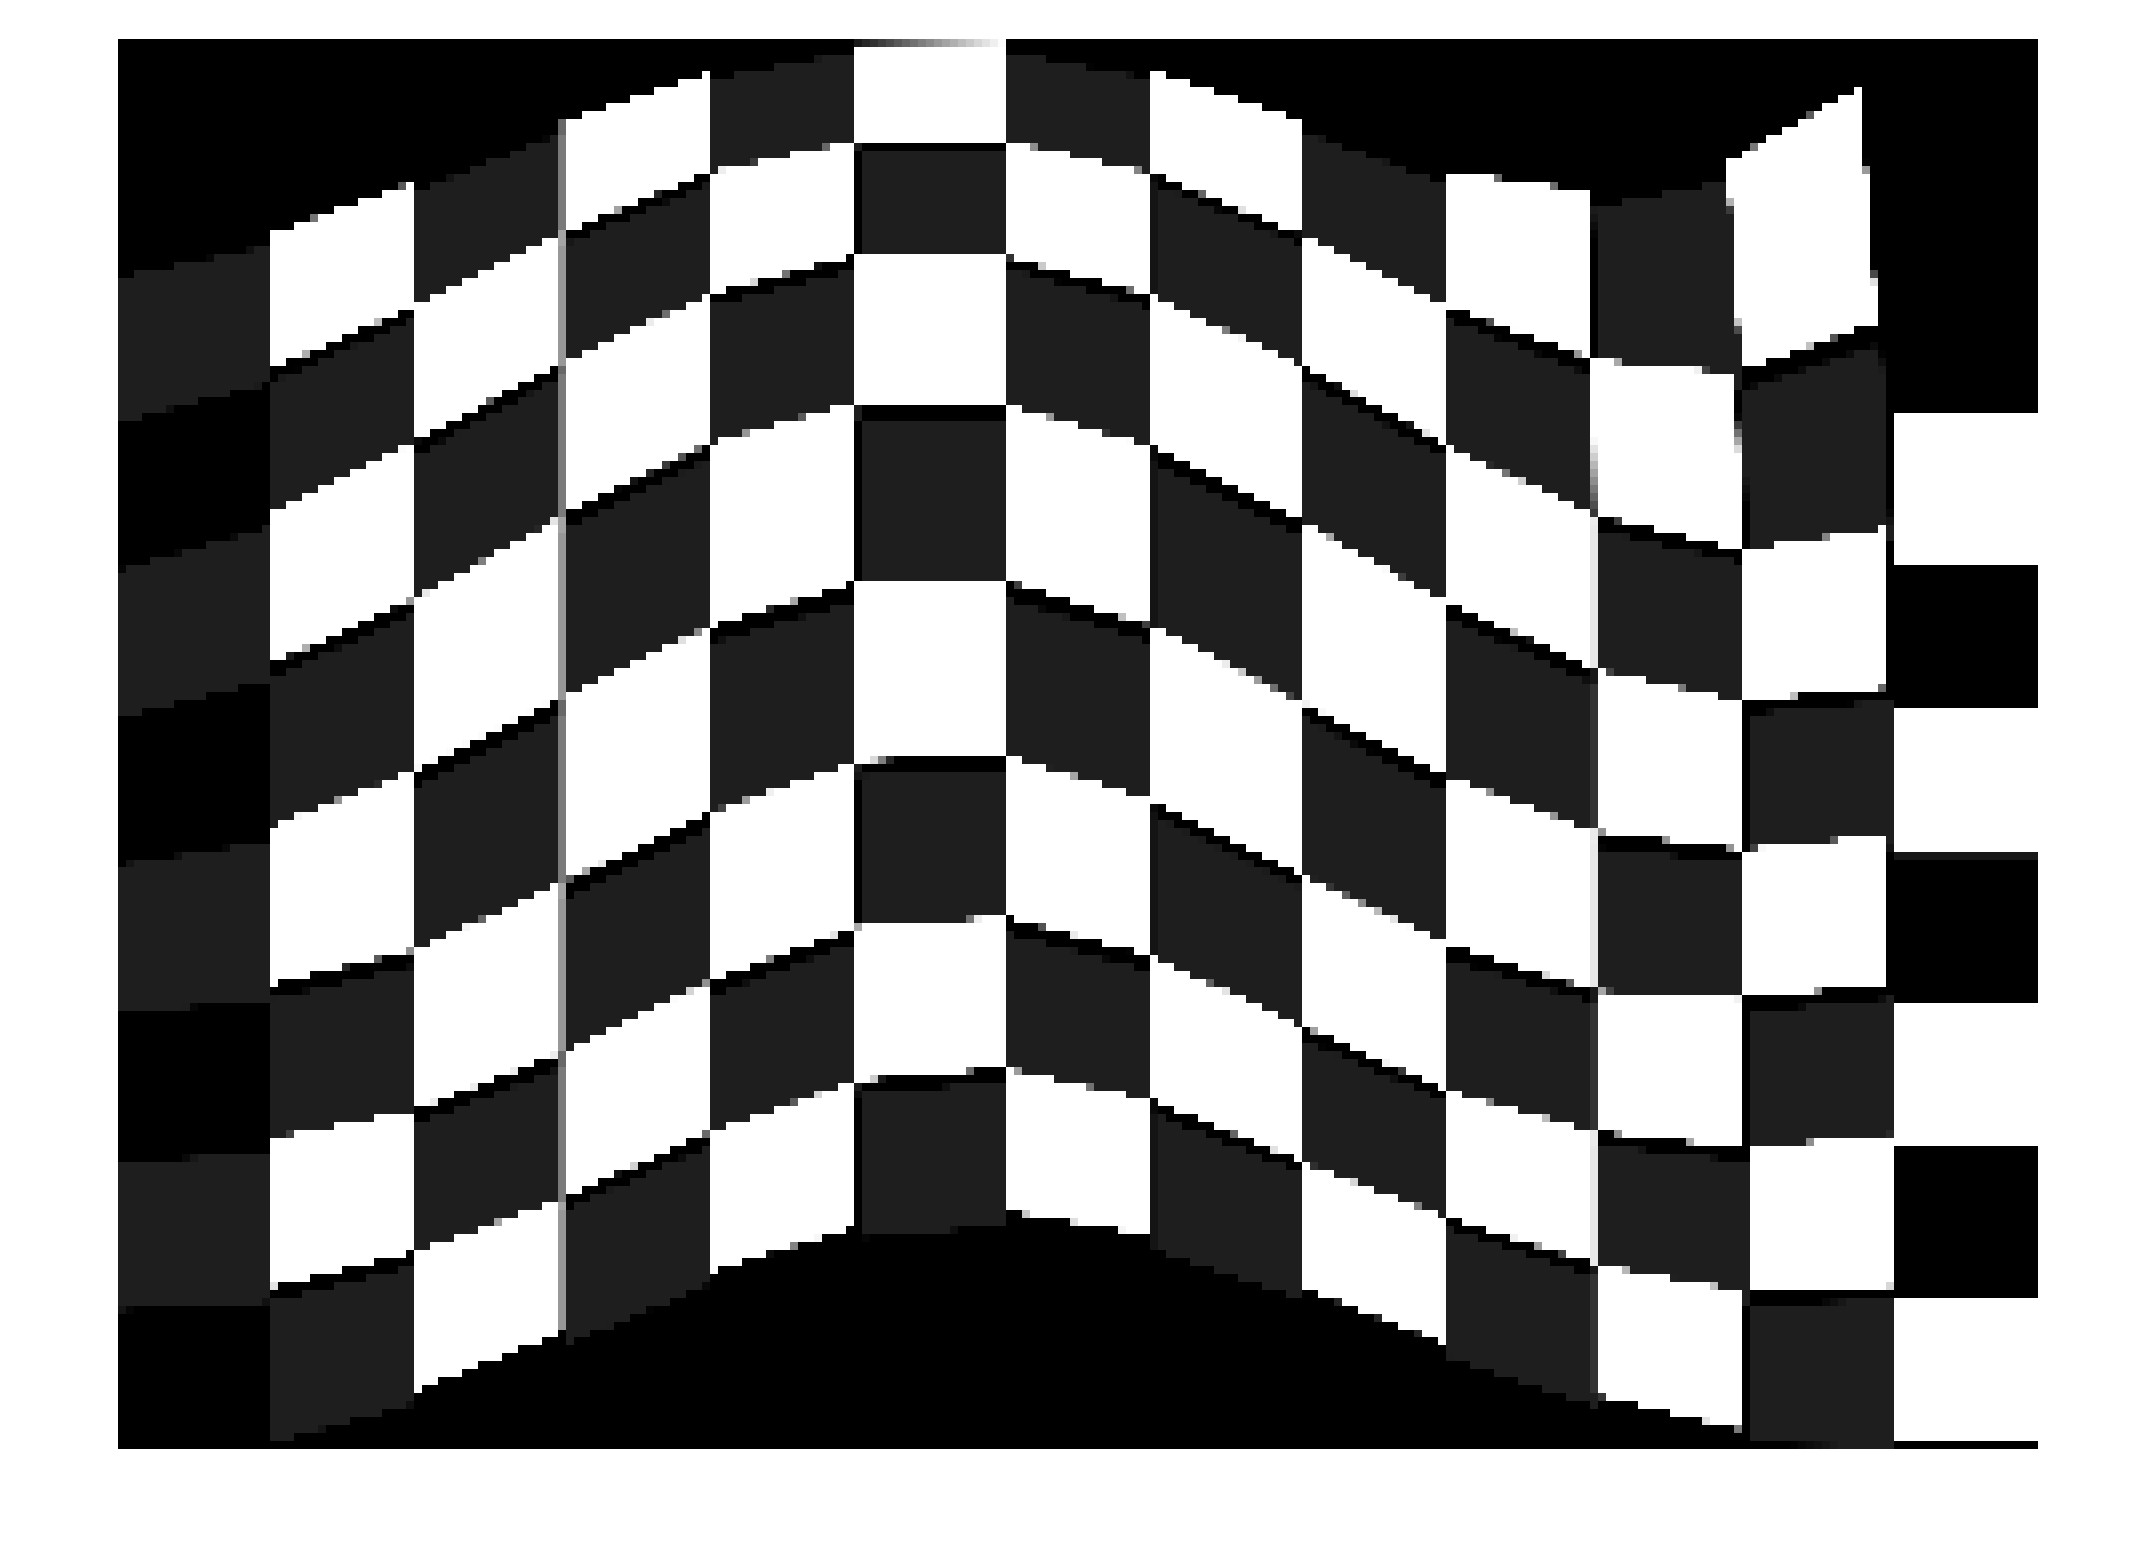
\includegraphics[scale=0.09]{interpolation_box.jpg}}
\end{figure}
What we can see from the results is that the nearest-neighbor and box sampling interpolation caused
more jaggy on the sampled graph. That is because that the nearest-neighbor interpolation 
calculates the average or closest value of each pixel and replaces it with the closest matching pixel and intensity value, 
resampling into the render's output, allows sharper detail. The box sampling will intensify the edge and overcome a scaling threshold on bilinear and bicubic interpolation
that results in lost data and fidelity when the algorithms include non-adjacent pixels in the sample, 
leading to imperfect results with artifacting and distortion.\par
3. Filter before sampling
We use PSF and Gauss function to filter out the graph then sample it.
\begin{figure}[H]
    \centering  %图片全局居中
    \subfigure[PSF]{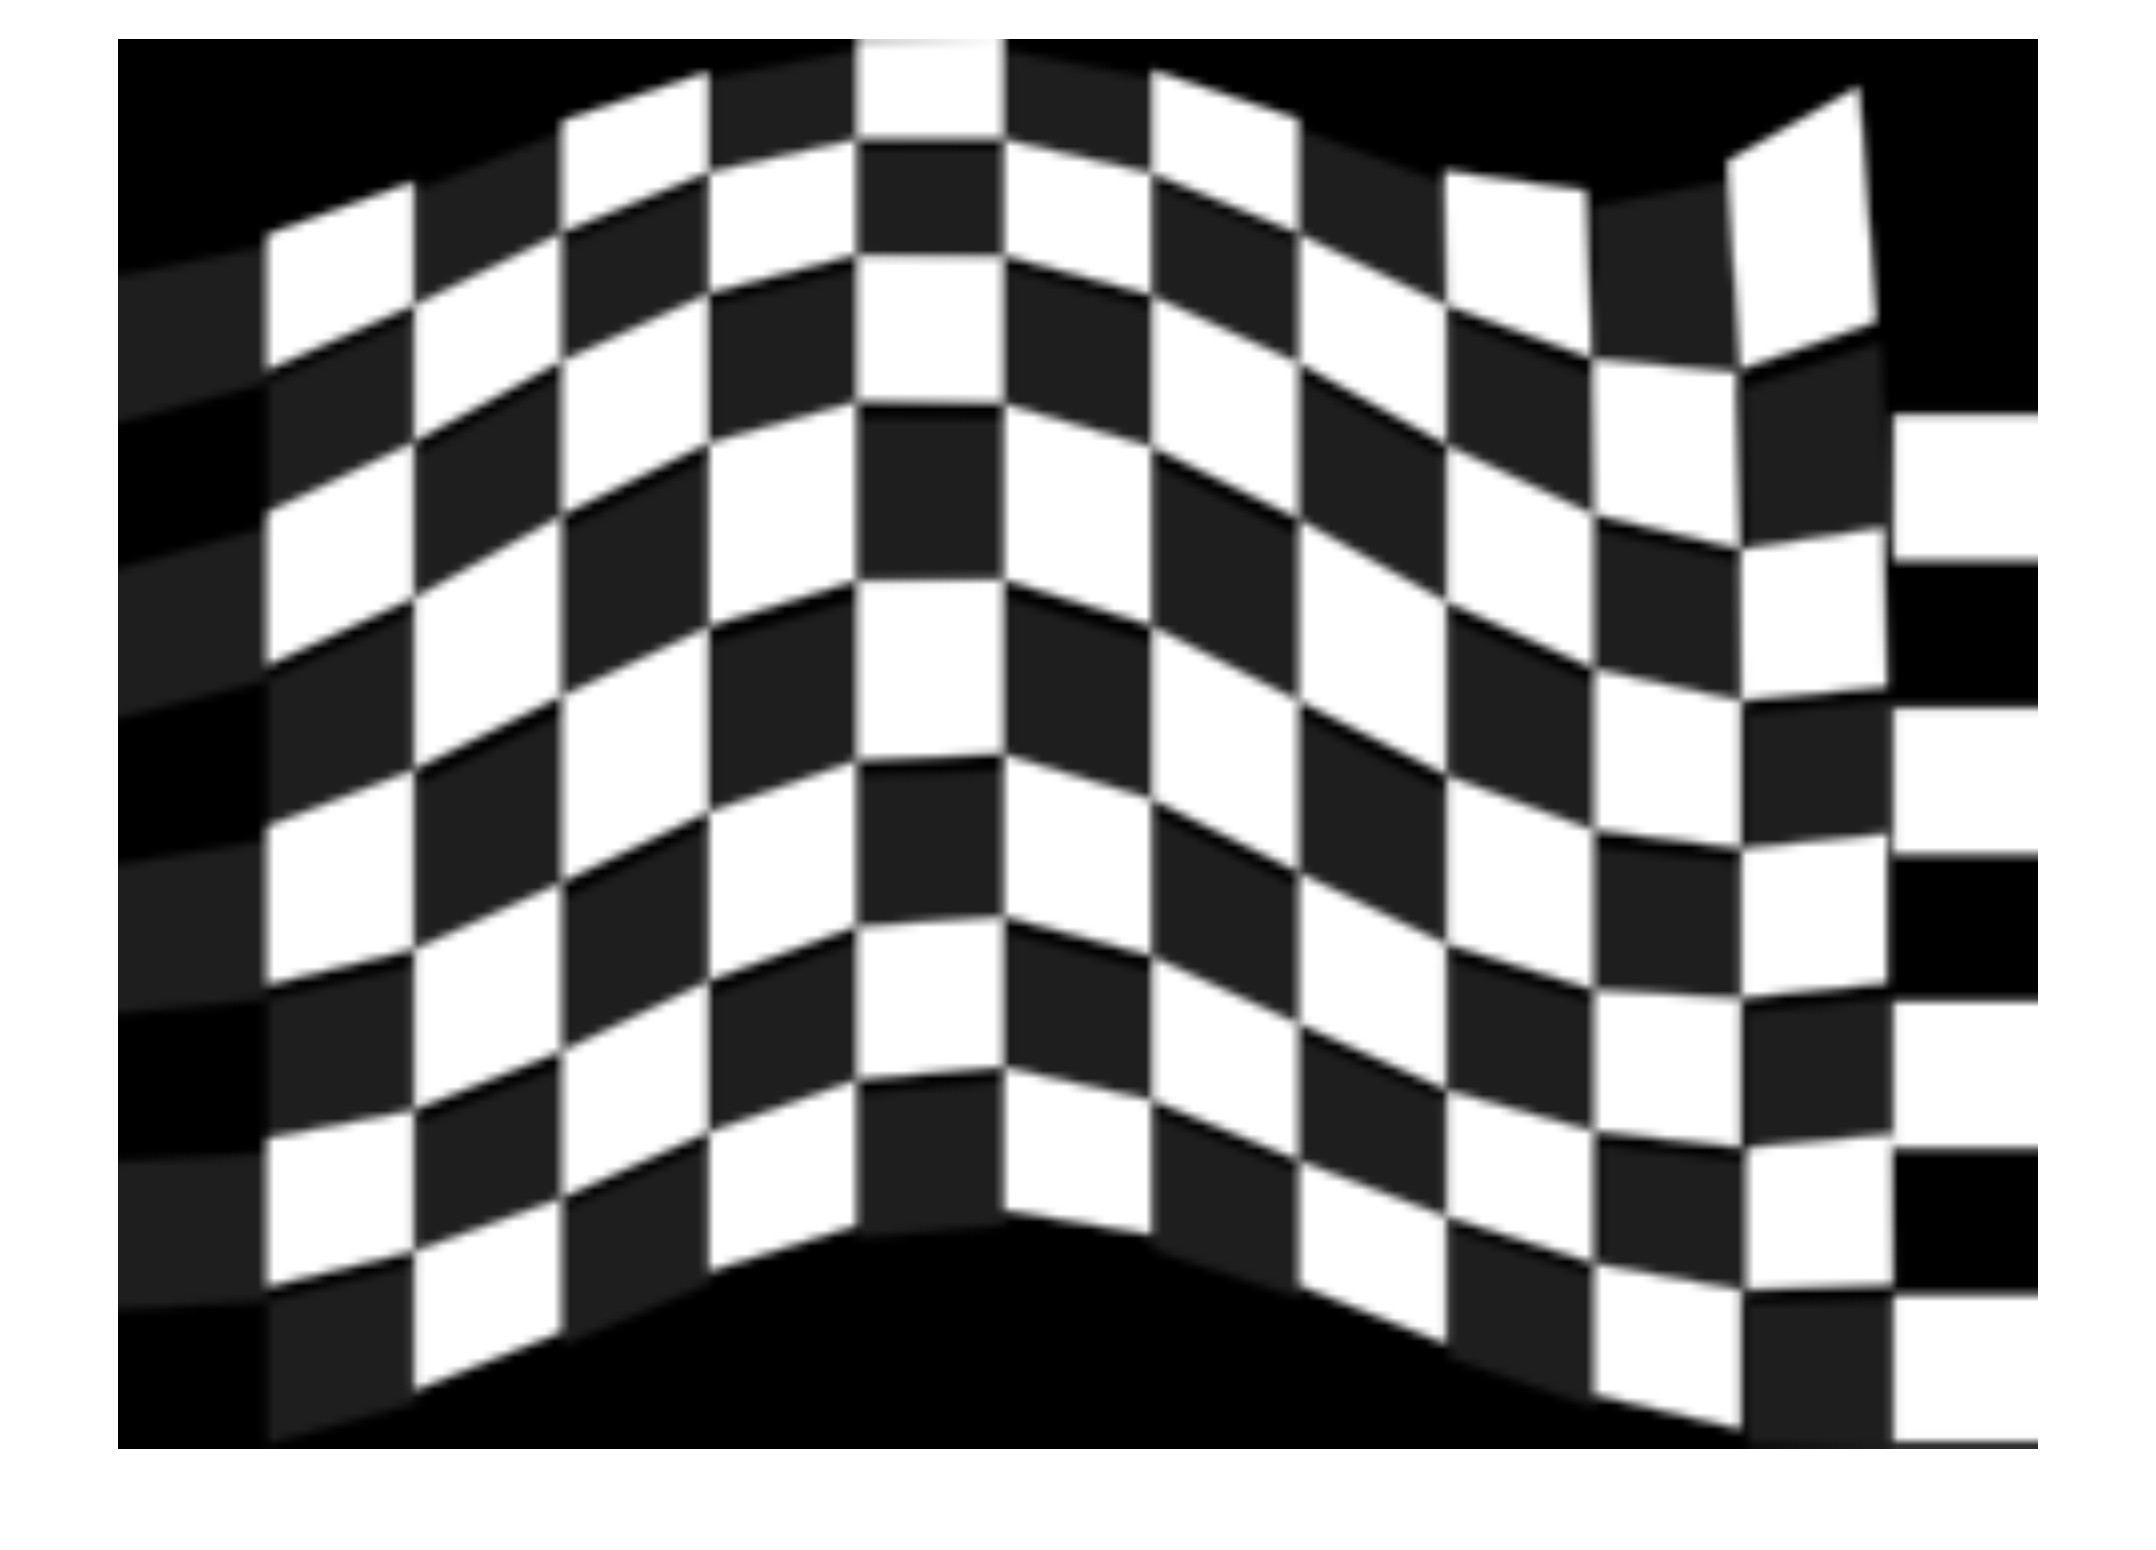
\includegraphics[scale=0.09]{PSF_Average_conv.jpg}}
    \subfigure[Gauss]{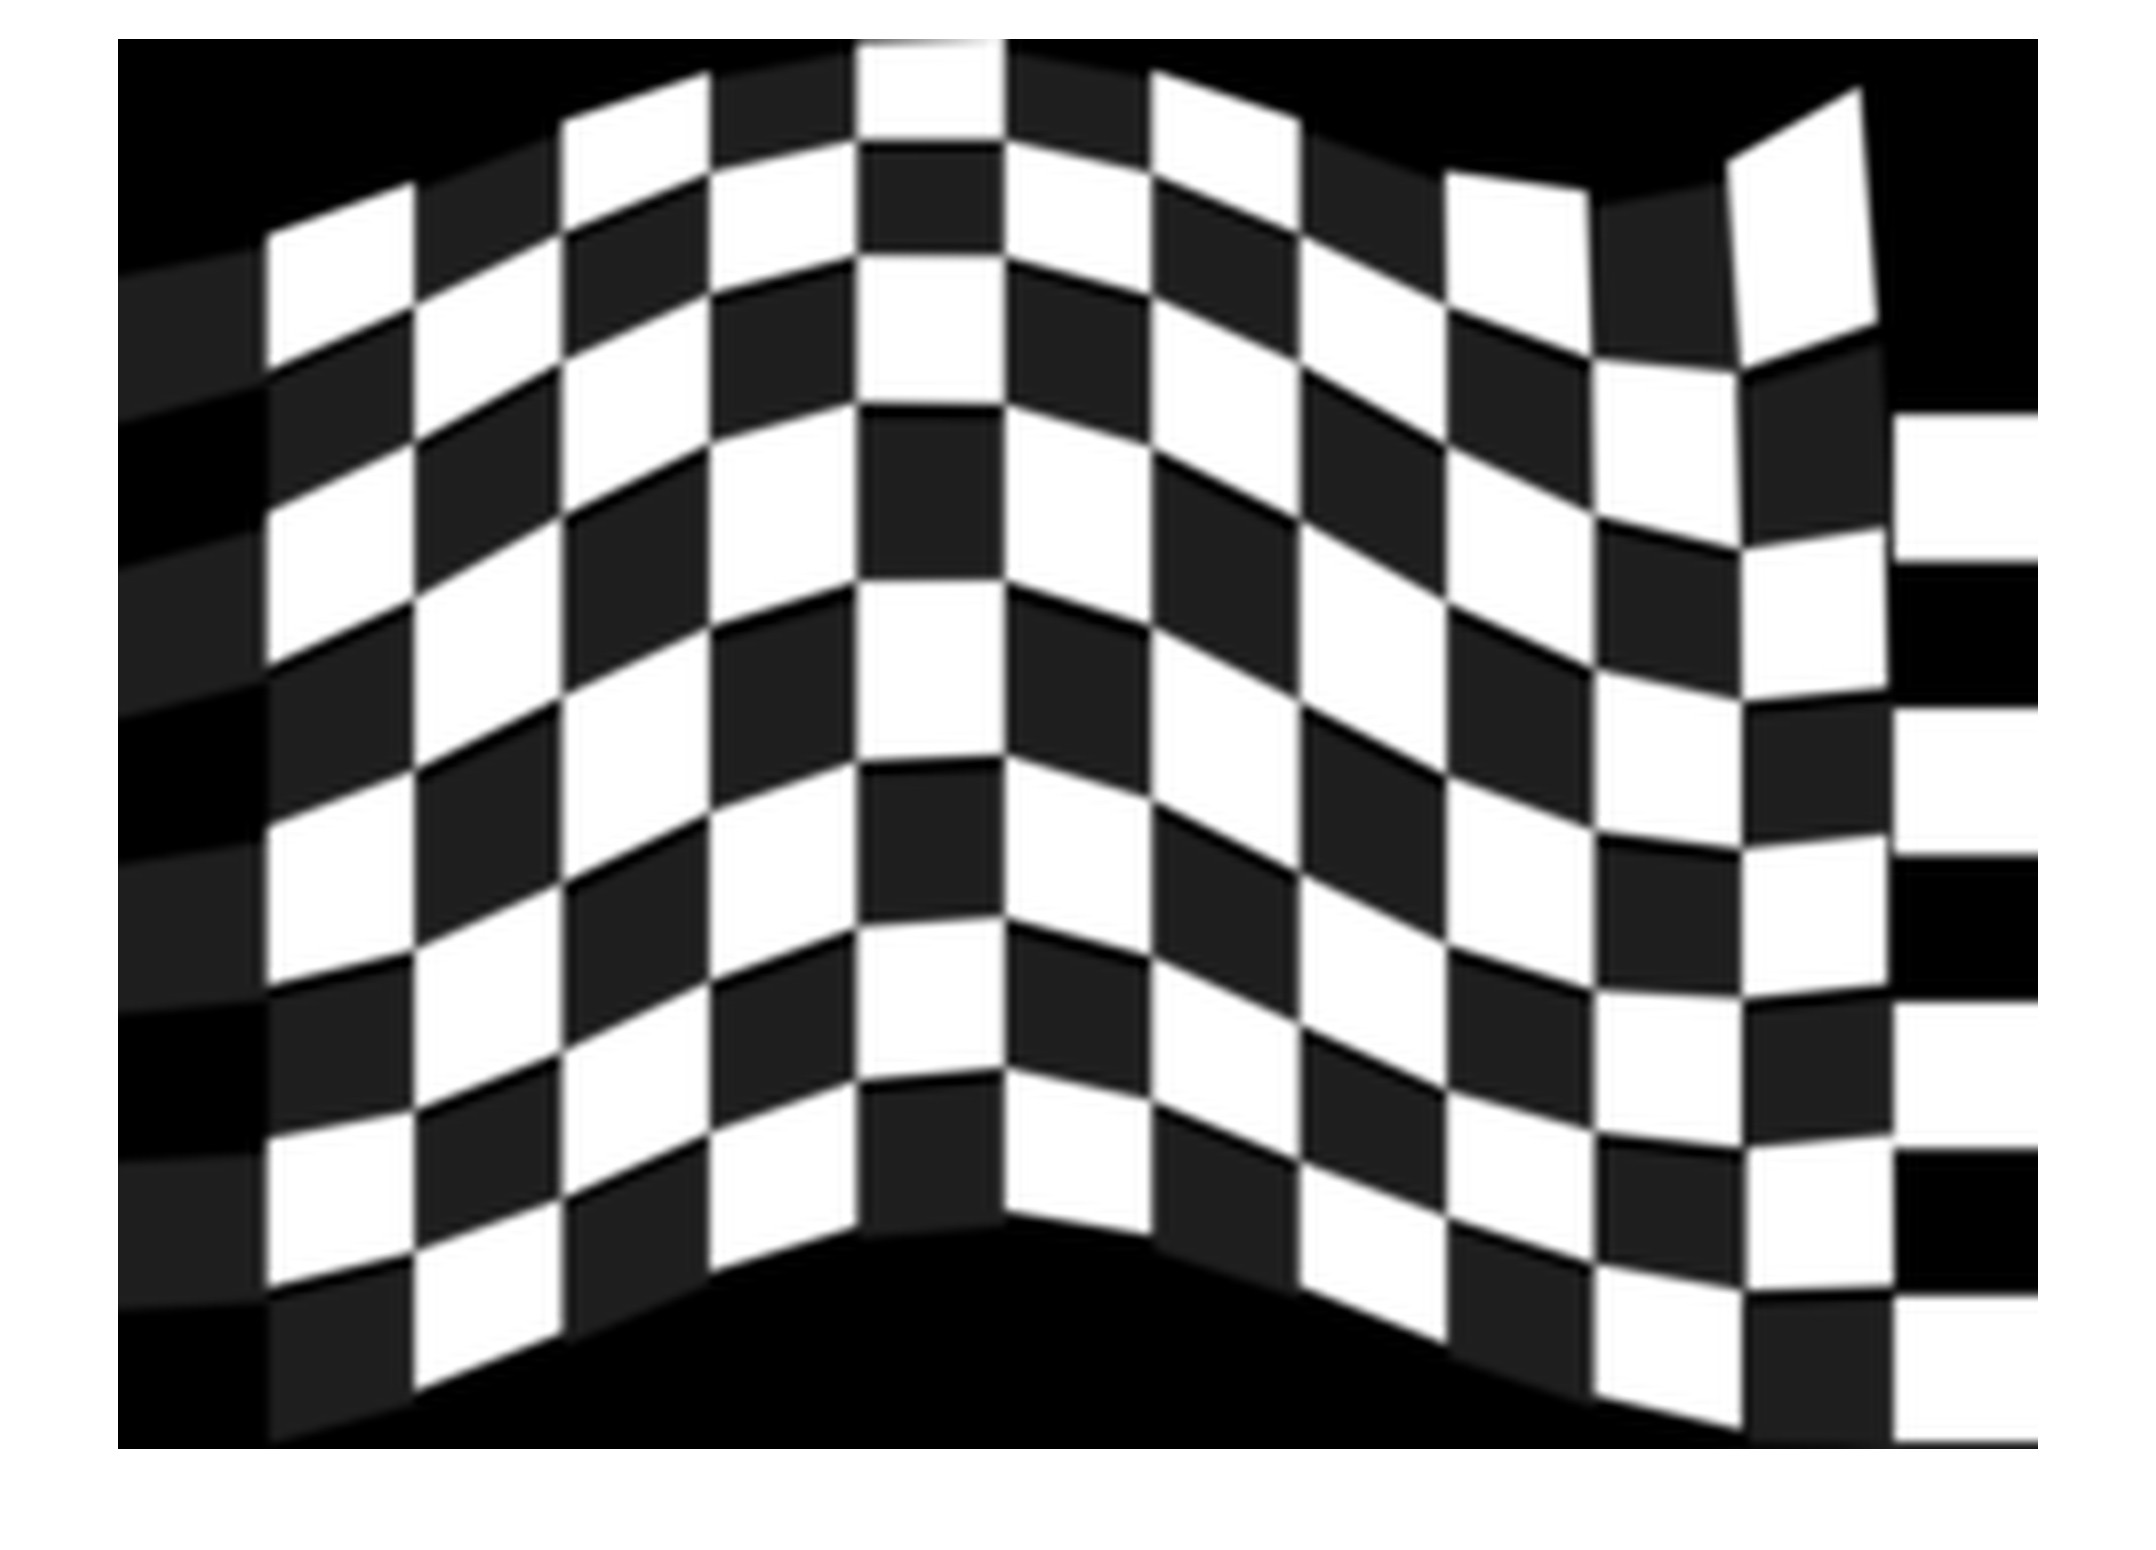
\includegraphics[scale=0.09]{gaussian_filter.jpg}}
\end{figure}
We can see that the anti-aliasing successfully on figure(i) and figure(j).
\clearpage
3. explanation on anti-aliasing.
A picture is a 2-D continuous time signal but it holds similar properties with the 1-D signal.
To interpret this, we can see that the edge between black blocks and white blocks has a rapid
change, that resembles to a high frequency components. And inside white or black blocks, the signal 
does not change or changed little so that they can be treated as low frequency components. \par
On 1-D signal, one of the most important property for us to decide whether it can be reconstruct 
after sampling is that sampling signal complies with Nyquist Sampling Theorem. When the signal is 
sampled with a signal, whose sampling frequency $\omega_s<2\omega_m$, the signal will have overlapped,
causing aliasing and distortion.
\begin{figure}[H]
\centering\subfigure[Illustrate of aliasing]{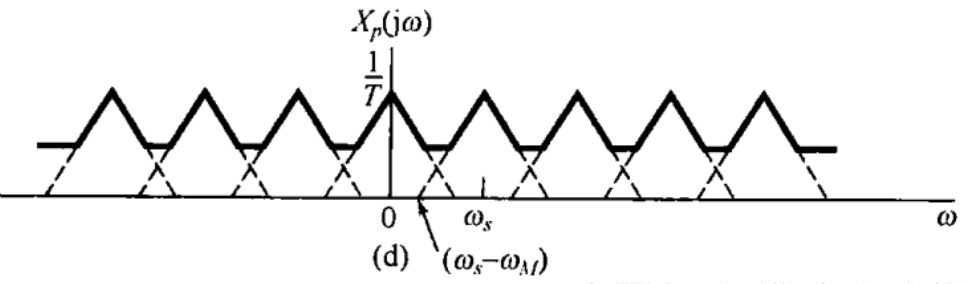
\includegraphics[scale=0.5]{alias.png}}
\subfigure[Illustrate of gaussian function]{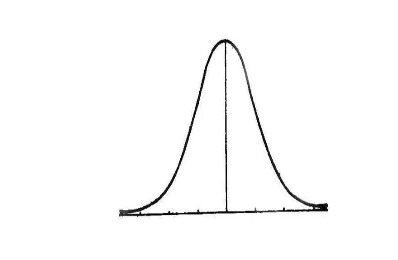
\includegraphics[scale=0.5]{Gauss.png}}
\end{figure}
So what we want to do is to is to eliminate the high frequency components from the graph before 
we sample so that we can counteract with some aliasing and decrease the jaggy phenomenon.\par
(1) Gaussian function: It has a normal form of $c\cdot e^{-at^2}$. So in frequency domain, we have:
\[
    \displaystyle F(j\omega)=\int_{-\infty}^{+\infty}e^{-at^2}e^{-j\omega t}dt=c\sqrt{\frac{\pi}{a}}e^{-\frac{w^2}{4a}}
\]
Obviously it is also a low pass filter. So that we can cut some components on high frequency and offset aliasing.\par
(2) Average convolution: This is a convolution method that we get the average number when the frequency changes too sharp 
at the edge of black and white blocks. So we can also reckon this as a low pass filter.\par
After let original signal(image) passed through a low pass filter, the picture will be obscured with less high frequency components.
Then the aliasing phenomenon will be alleviated.
\par
The experiment is carried out by matlab, using "Image Processing Toolbox".
\end{document}